\begin{figure*}[htbp] % *!
    \centering
    % --- Row 1 (P=2) ---
    % Label
    \parbox[c]{0.03\linewidth}{\centering \rotatebox{90}{$P = 2$}}%
    \hfill
    % Images with valign=c
    \subfloat[]{ 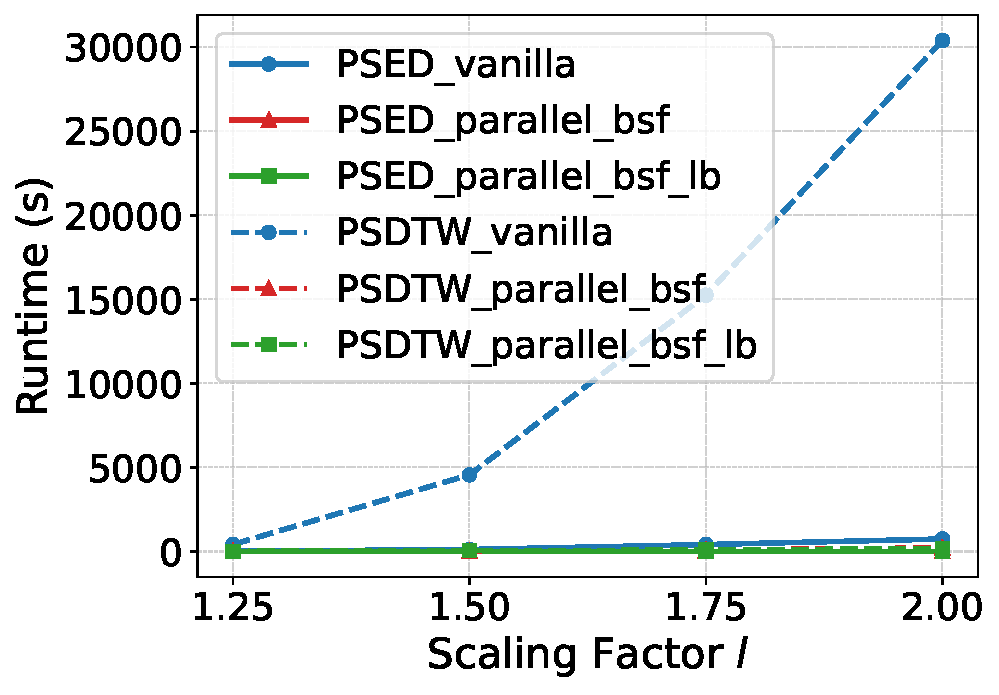
\includegraphics[width=0.21\linewidth, valign=c]{figures/gunpoint-runtime-P2-time.pdf} } \hfill
    \subfloat[]{ 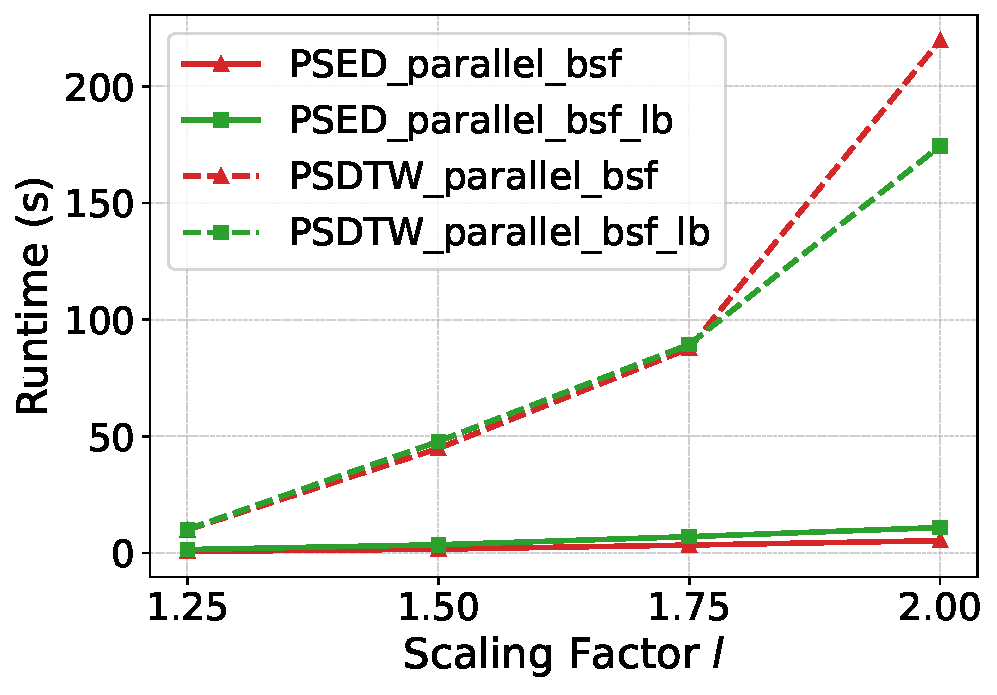
\includegraphics[width=0.21\linewidth, valign=c]{figures/gunpoint-runtime-P2-focus-time.pdf} } \hfill
    \subfloat[]{ 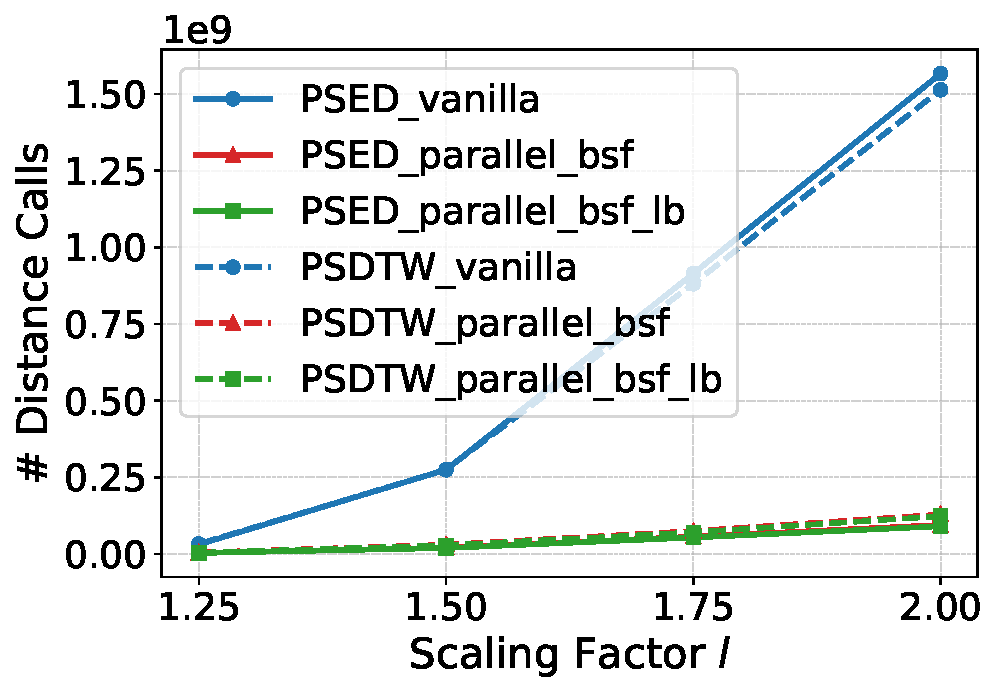
\includegraphics[width=0.21\linewidth, valign=c]{figures/gunpoint-runtime-P2-distance-call.pdf} } \hfill
    \subfloat[]{ 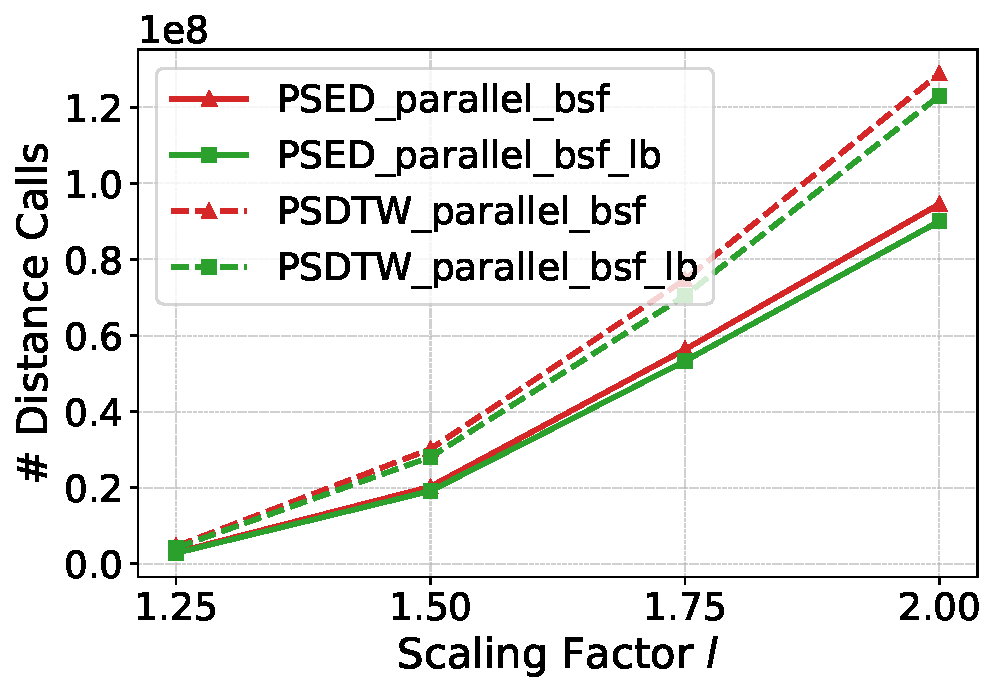
\includegraphics[width=0.21\linewidth, valign=c]{figures/gunpoint-runtime-P2-focus-distance-call.pdf} }
    
    \par \vspace{0.2cm} 
    
    % --- Row 2 (P=3) ---
    % Label
    \parbox[c]{0.03\linewidth}{\centering \rotatebox{90}{$P = 3$}}%
    \hfill
    % Images with valign=c
    \subfloat[]{ 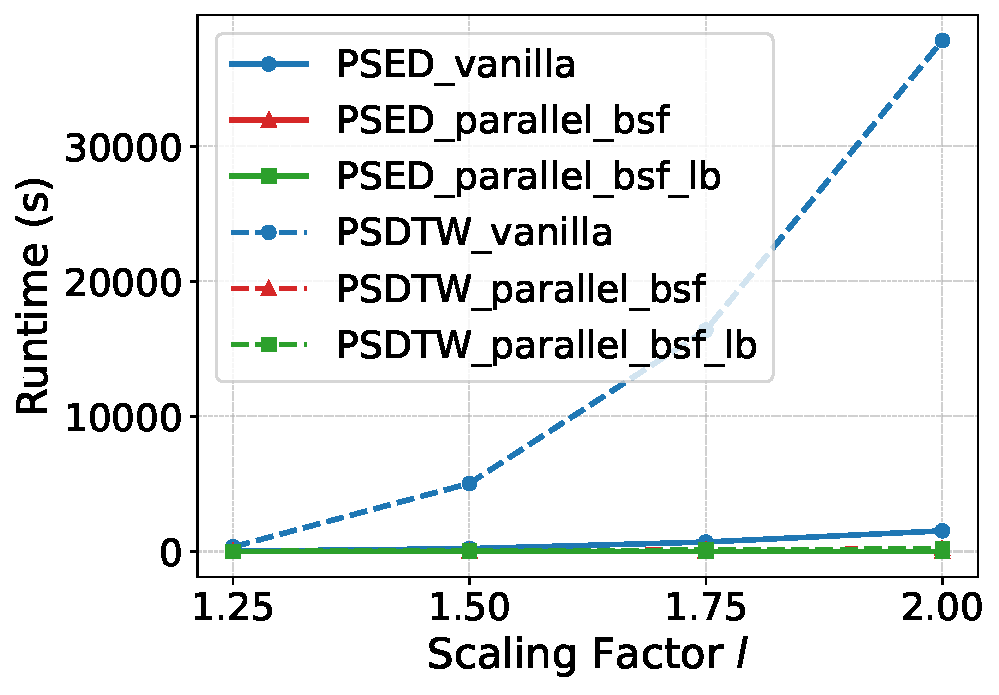
\includegraphics[width=0.21\linewidth, valign=c]{figures/gunpoint-runtime-P3-time.pdf} } \hfill
    \subfloat[]{ 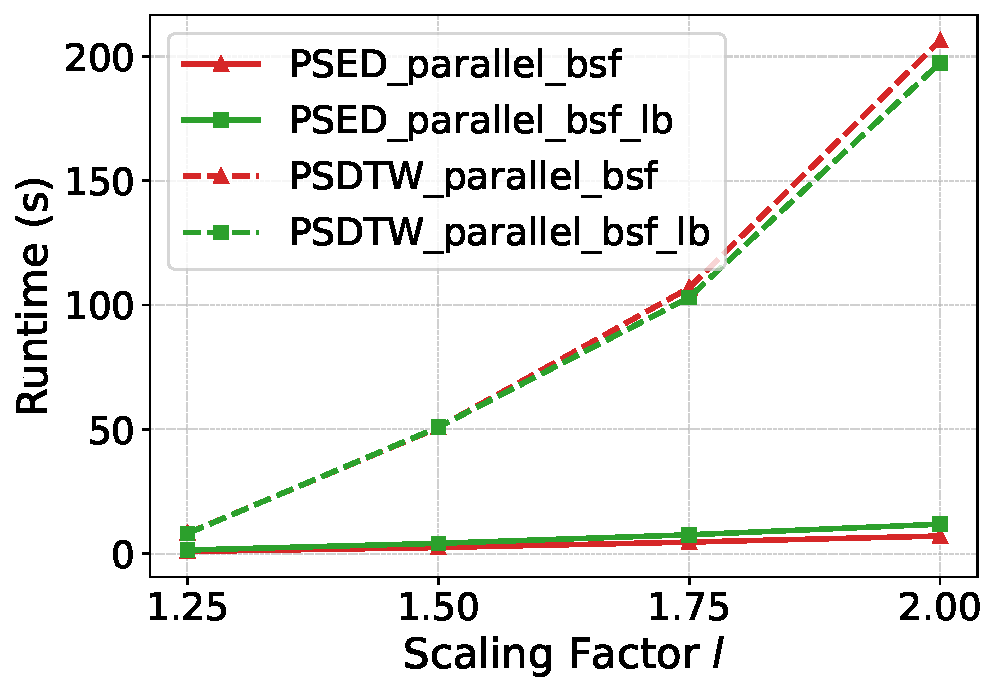
\includegraphics[width=0.21\linewidth, valign=c]{figures/gunpoint-runtime-P3-focus-time.pdf} } \hfill
    \subfloat[]{ 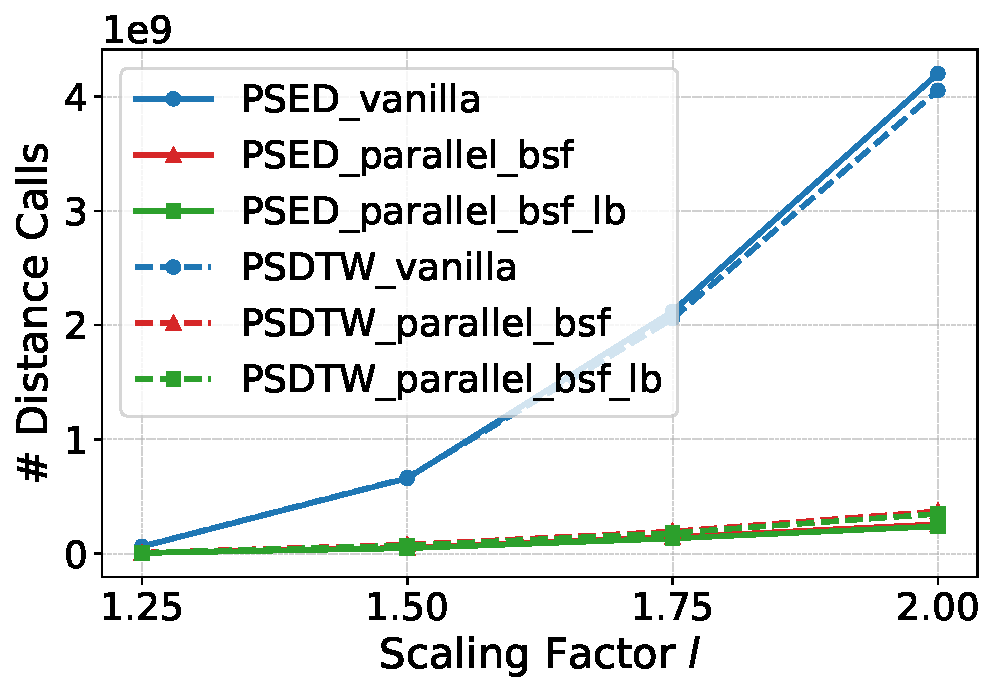
\includegraphics[width=0.21\linewidth, valign=c]{figures/gunpoint-runtime-P3-distance-call.pdf} } \hfill
    \subfloat[]{ 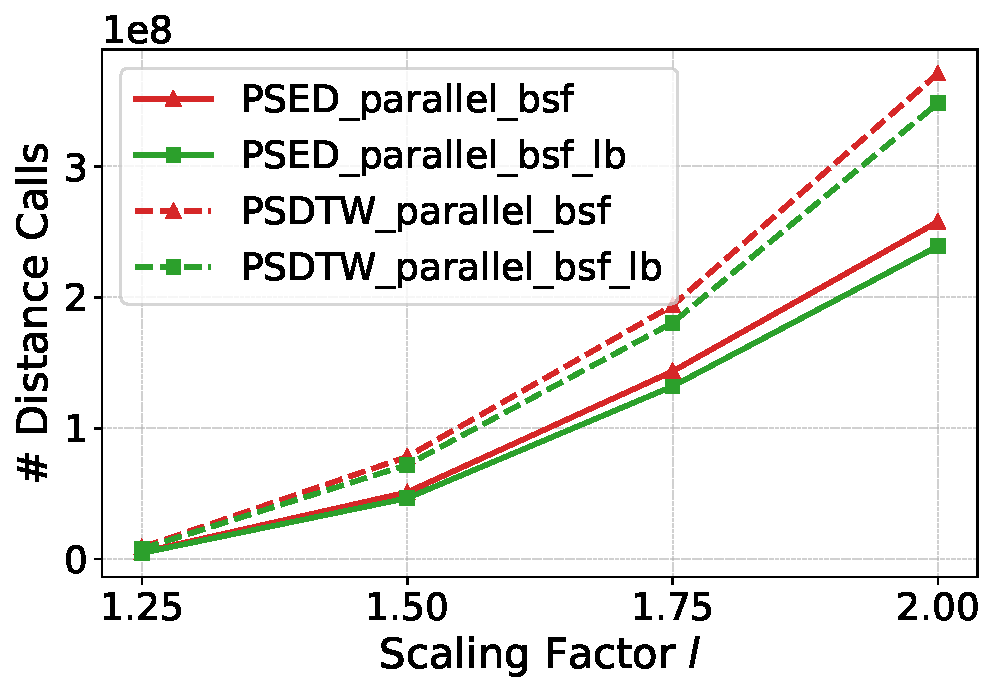
\includegraphics[width=0.21\linewidth, valign=c]{figures/gunpoint-runtime-P3-focus-distance-call.pdf} }
    
    \par \vspace{0.2cm} 
    
    % --- Row 3 (P=4) ---
    % Label
    \parbox[c]{0.03\linewidth}{\centering \rotatebox{90}{$P = 4$}}%
    \hfill
    % Images with valign=c
    \subfloat[]{ 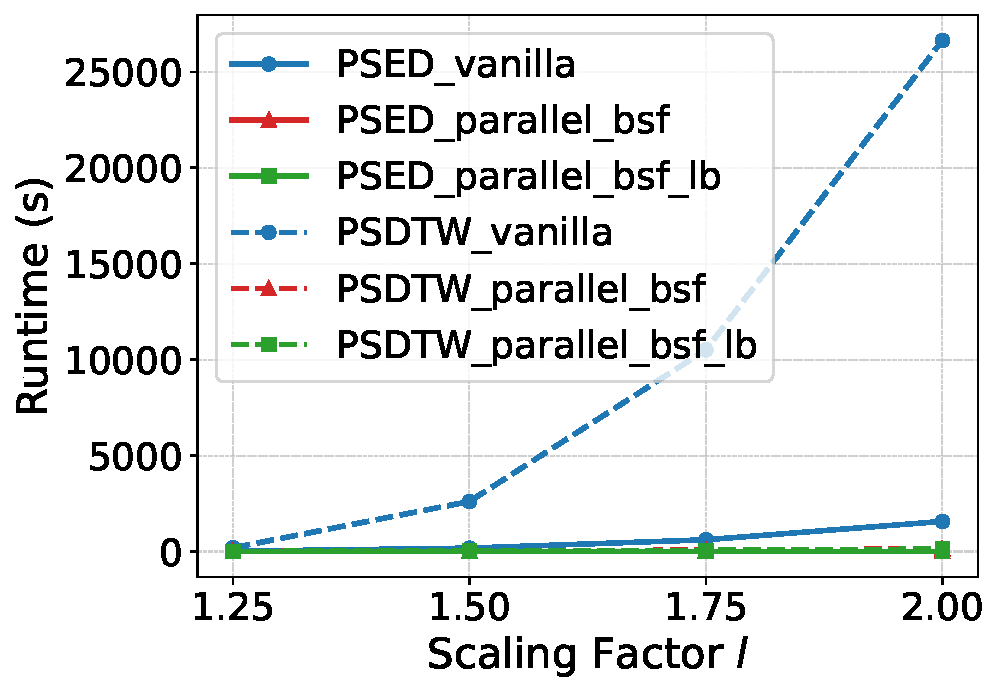
\includegraphics[width=0.21\linewidth, valign=c]{figures/gunpoint-runtime-P4-time.pdf} } \hfill
    \subfloat[]{ 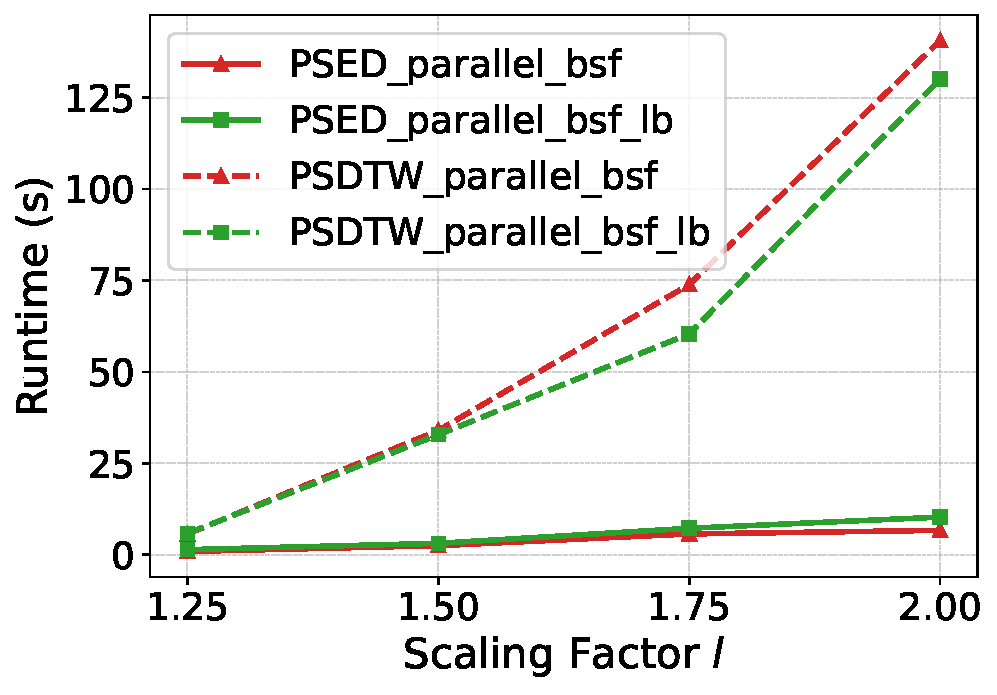
\includegraphics[width=0.21\linewidth, valign=c]{figures/gunpoint-runtime-P4-focus-time.pdf} } \hfill
    \subfloat[]{ 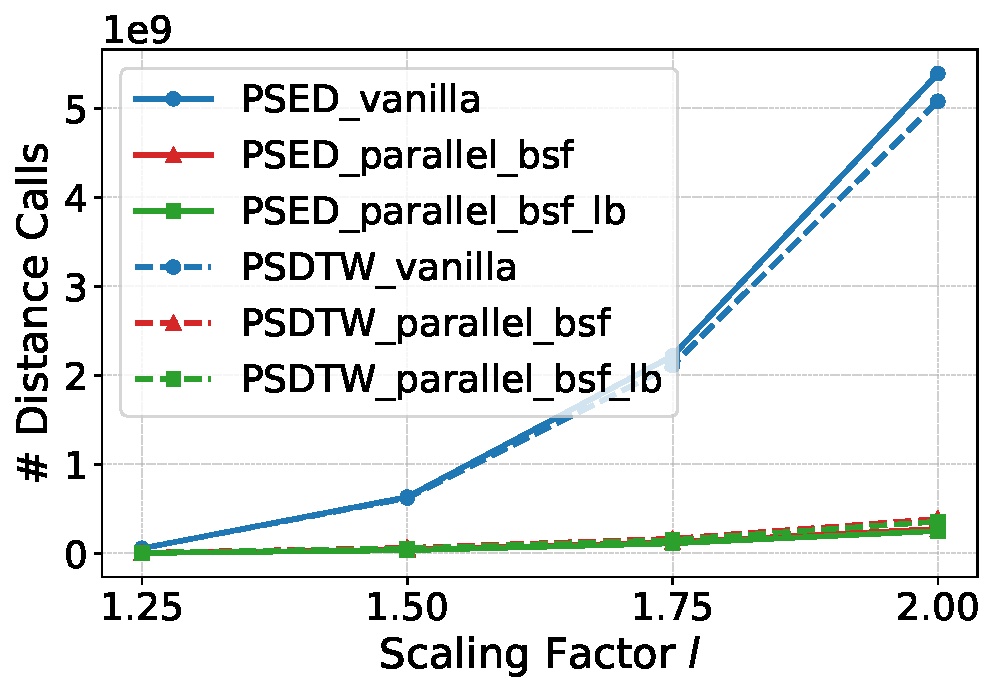
\includegraphics[width=0.21\linewidth, valign=c]{figures/gunpoint-runtime-P4-distance-call.pdf} } \hfill
    \subfloat[]{ 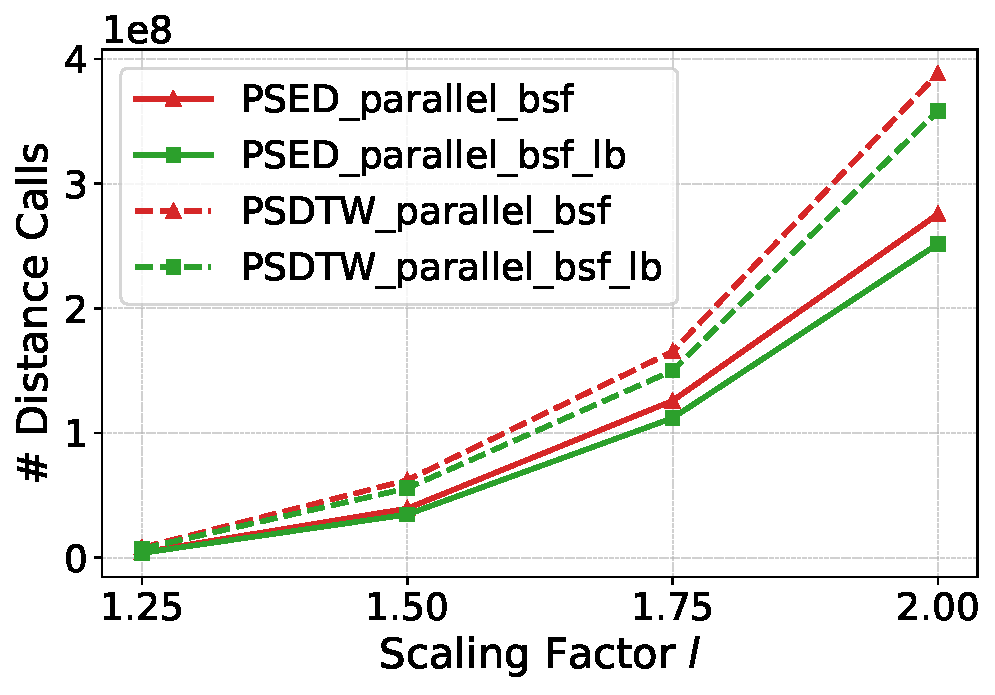
\includegraphics[width=0.21\linewidth, valign=c]{figures/gunpoint-runtime-P4-focus-distance-call.pdf} }

    \caption{Comparing runtime and the number of distance calls for the methods with different $P$ and $l$ on the GunPoint dataset.}
    \label{fig:gunpoint-runtime}
\end{figure*}